\documentclass[12pt, a4paper]{article}

% ── Packages ──────────────────────────────────────────────────────────────────
\usepackage[margin=2.5cm]{geometry}
\usepackage{amsmath, amssymb, amsthm}
\usepackage{mathtools}
\usepackage{graphicx}
\usepackage{xcolor}
\usepackage{booktabs}
\usepackage{array}
\usepackage{tabularx}
\usepackage{enumitem}
\usepackage{hyperref}
\usepackage{cite}
\usepackage{fancyhdr}
\usepackage{titlesec}
\usepackage{microtype}
\usepackage{setspace}
\usepackage{caption}
\usepackage{subcaption}
\usepackage{tcolorbox}
\usepackage{tikz}
\usepackage{float}
\usepackage{parskip}
\usepackage{mdframed}

% ── Colours ───────────────────────────────────────────────────────────────────
\definecolor{deepblue}{HTML}{1565C0}
\definecolor{midblue}{HTML}{1976D2}
\definecolor{lightblue}{HTML}{E3F2FD}
\definecolor{darkgrey}{HTML}{1a1a2e}
\definecolor{medgrey}{HTML}{546E7A}
\definecolor{accentred}{HTML}{C62828}
\definecolor{accentgreen}{HTML}{2E7D32}
\definecolor{boxbg}{HTML}{F8F9FA}
\definecolor{boxborder}{HTML}{1565C0}

% ── Hyperref setup ─────────────────────────────────────────────────────────────
\hypersetup{
  colorlinks=true,
  linkcolor=deepblue,
  citecolor=accentred,
  urlcolor=midblue,
  pdftitle={ECG Biometric Identification via WTMM Representations},
  pdfauthor={Manuscript}
}

% ── Section formatting ─────────────────────────────────────────────────────────
\titleformat{\section}
  {\large\bfseries\color{deepblue}}{\thesection.}{0.6em}{}[\vspace{-0.3em}\textcolor{deepblue}{\rule{\linewidth}{0.6pt}}]

\titleformat{\subsection}
  {\normalsize\bfseries\color{darkgrey}}{\thesubsection}{0.6em}{}

\titleformat{\subsubsection}
  {\normalsize\itshape\color{medgrey}}{\thesubsubsection}{0.6em}{}

% ── Header / footer ────────────────────────────────────────────────────────────
\pagestyle{fancy}
\fancyhf{}
\fancyhead[L]{\small\color{medgrey}\textit{ECG Biometrics via Wavelet Transform Modulus Maxima}}
\fancyhead[R]{\small\color{medgrey}\textit{Manuscript --- Under Review}}
\fancyfoot[C]{\small\color{medgrey}\thepage}
\renewcommand{\headrulewidth}{0.4pt}
\renewcommand{\headrule}{\hbox to\headwidth{\color{deepblue}\leaders\hrule height \headrulewidth\hfill}}

% ── Math operators ─────────────────────────────────────────────────────────────
\DeclareMathOperator{\sgn}{sgn}
\DeclareMathOperator{\E}{\mathbb{E}}
\newcommand{\R}{\mathbb{R}}
\newcommand{\norm}[1]{\left\lVert#1\right\rVert}
\newcommand{\abs}[1]{\left|#1\right|}
\newcommand{\inner}[2]{\langle #1,\, #2 \rangle}
\newcommand{\scalogram}{\mathcal{S}}
\newcommand{\CWT}{\mathcal{W}}

% ── Coloured math box ──────────────────────────────────────────────────────────
\newmdenv[
  backgroundcolor=lightblue,
  linecolor=boxborder,
  linewidth=1.2pt,
  leftmargin=0pt, rightmargin=0pt,
  innerleftmargin=12pt, innerrightmargin=12pt,
  innertopmargin=8pt, innerbottommargin=8pt,
  skipabove=8pt, skipbelow=8pt
]{mathbox}

% ── Figure placeholder ─────────────────────────────────────────────────────────
\newcommand{\figplaceholder}[2]{%
  \begin{figure}[H]
    \centering
    \begin{tikzpicture}
      \draw[dashed, color=medgrey, line width=0.8pt, rounded corners=4pt]
        (0,0) rectangle (#1);
      \node[color=medgrey, font=\small\itshape] at ({#1/2 - 1.5cm}, {#1*0.25}) {#2};
    \end{tikzpicture}
  \end{figure}
}

% ── Caption style ──────────────────────────────────────────────────────────────
\captionsetup{font=small, labelfont={bf,color=deepblue}, textfont=it,
              margin=1cm, skip=6pt}

% ─────────────────────────────────────────────────────────────────────────────
\begin{document}

% ════════════════════════════════════════════════════════════════════════════════
%  TITLE BLOCK
% ════════════════════════════════════════════════════════════════════════════════
\begin{center}
  {\LARGE\bfseries\color{deepblue}
    ECG-Based Biometric Identification via\\[4pt]
    Wavelet Transform Modulus Maxima Representations
  }\\[10pt]
  {\large\color{medgrey}
    Comparing Classical and Neural One-Class Models
  }\\[16pt]
  {\normalsize [Author Names Redacted for Review]}\\[4pt]
  {\small\color{medgrey}
    Department of Biomedical Engineering \quad $\cdot$ \quad [Institution]\\
    Correspondence: \texttt{[email@institution.edu]}
  }\\[8pt]
  \textcolor{deepblue}{\rule{0.6\linewidth}{0.8pt}}
\end{center}

\vspace{6pt}

% ── Abstract ───────────────────────────────────────────────────────────────────
\begin{tcolorbox}[
  colback=lightblue, colframe=deepblue,
  boxrule=0.8pt, arc=4pt,
  left=12pt, right=12pt, top=8pt, bottom=8pt
]
  \textbf{\color{deepblue}Abstract.}\quad
  Electrocardiogram (ECG) signals carry unique, body-internal patterns
  that make them a compelling biometric modality --- one that is naturally
  tied to liveness and difficult to spoof.
  %
  In this work, we transform raw ECG recordings into two-dimensional
  time--frequency images using the Continuous Wavelet Transform (CWT)
  with a Morlet mother wavelet, and then extract a compact,
  scale-structured representation through the
  \textit{Wavelet Transform Modulus Maxima} (WTMM) method.
  %
  These skeletal images are fed into six one-class classification
  frameworks: One-Class SVM, Isolation Forest, Local Outlier Factor,
  Gaussian Mixture Model, PCA reconstruction, and a
  \textit{Kolmogorov--Arnold Network} (KAN) autoencoder.
  %
  Using the publicly available ECG-ID database, we evaluate each model
  on its ability to accept genuine heartbeats while rejecting impostors,
  reporting AUROC, precision--recall, true positive rate, and true
  negative rate. Our results confirm that wavelet-based representations
  preserve discriminative cardiac morphology, and we discuss the
  comparative performance of classical and modern neural approaches.
  We also raise open questions about liveness definitions in
  physiological biometrics.\\[4pt]
  \textbf{\color{deepblue}Keywords:}~
  ECG biometrics; wavelet transform; WTMM; Morlet wavelet;
  one-class classification; Kolmogorov--Arnold networks; liveness detection.
\end{tcolorbox}

\vspace{10pt}

% ════════════════════════════════════════════════════════════════════════════════
%  1. INTRODUCTION
% ════════════════════════════════════════════════════════════════════════════════
\section{Introduction}

Biometric authentication has come a long way from fingerprints and iris
scans. While these modalities work well in controlled settings, they share
a common weakness: the features they measure sit on the surface of the body,
where they can --- in principle --- be copied, replayed, or tricked.
A fingerprint can be lifted from a glass; a face can be spoofed with a
photograph or a mask.
In contrast, \textit{bioelectric signals} such as the
electroencephalogram (EEG) and electrocardiogram (ECG) originate deep inside
the body and reflect anatomy that cannot easily be reproduced from the outside.
The ECG, in particular, is generated only by a beating, living heart, giving
it an \textit{inherent liveness property} that surface-based modalities simply
do not have~\cite{he2022,byeon2019}.

What makes the ECG attractive as a biometric? At its core, the cardiac
electrical cycle (the well-known PQRST waveform, illustrated in
Figure~\ref{fig:pqrst_placeholder}) is shaped by the geometry of the heart
muscle, the conductivity of surrounding tissue, and the organisation of the
electrical conduction system. All of these differ between individuals in
measurable, reproducible ways. The result is a signal that is both
\textit{unique} (different people produce different patterns) and
\textit{stable} (the same person produces consistent patterns over time
under resting conditions)~\cite{he2022}.

There are practical advantages too. Modern wearable devices --- smartwatches,
fitness bands, even ECG-capable rings --- can record a one-lead ECG
continuously and passively.
This opens the door to \textit{continuous authentication}: a system that
keeps verifying the user's identity in the background, not just at login
time~\cite{bhuva2023}.

Despite these appealing properties, turning an ECG waveform into a reliable
biometric feature is a genuine signal-processing challenge.
The raw ECG is a one-dimensional, non-stationary time series. Its
frequency content evolves during the cardiac cycle: the sharp QRS complex
concentrates energy in the 10--40~Hz range, while the gentler P and T waves
sit mostly below 5~Hz. A representation that captures only time (e.g., a raw
sample window) or only frequency (e.g., a power spectrum) loses important
structure.

This motivates a \textit{time--frequency} approach. In this paper, we apply
the Continuous Wavelet Transform (CWT) with a Morlet mother wavelet to extract
scalogram images from individual heartbeat cycles, and then go one step further
by computing the \textit{Wavelet Transform Modulus Maxima} (WTMM) skeleton ---
a sparse, structured summary of the most important transient events in each
beat. These WTMM images are then fed into six one-class classification
models, ranging from the well-established One-Class SVM to the recently
proposed Kolmogorov--Arnold Network (KAN).

The remainder of the paper is organised as follows.
Section~\ref{sec:related} reviews related work on ECG biometrics and
time--frequency representations.
Section~\ref{sec:dataset} describes the ECG-ID database.
Section~\ref{sec:methods} presents the full signal-processing and feature-
extraction pipeline with mathematical details.
Section~\ref{sec:models} describes the classification models.
Section~\ref{sec:experiments} reports experimental results.
Section~\ref{sec:discussion} discusses findings and open questions.
Section~\ref{sec:conclusion} concludes.

% ── Figure 1 placeholder ──────────────────────────────────────────────────────
\begin{figure}[H]
  \centering
  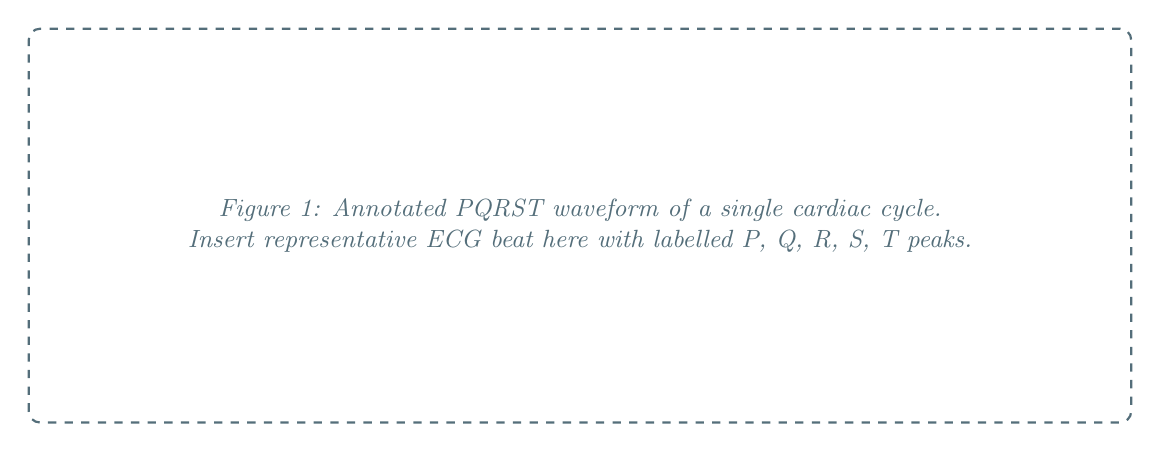
\begin{tikzpicture}
    \draw[dashed, color=medgrey, line width=0.8pt, rounded corners=4pt]
      (0,0) rectangle (14cm, 5cm);
    \node[color=medgrey, font=\small\itshape, align=center] at (7cm, 2.5cm)
      {Figure 1: Annotated PQRST waveform of a single cardiac cycle.\\
       Insert representative ECG beat here with labelled P, Q, R, S, T peaks.};
  \end{tikzpicture}
  \caption{A single cardiac cycle showing the canonical PQRST deflections.
    The sharp R peak serves as the temporal anchor for beat segmentation.
    Differences in amplitude, duration, and morphology of these features
    across individuals provide the discriminative information exploited by
    biometric models.}
  \label{fig:pqrst_placeholder}
\end{figure}

% ════════════════════════════════════════════════════════════════════════════════
%  2. RELATED WORK
% ════════════════════════════════════════════════════════════════════════════════
\section{Related Work}
\label{sec:related}

\subsection{ECG as a Biometric}

The idea of using the ECG for person identification goes back at least to the
early 2000s, when Israel~et~al.~\cite{israel2005} demonstrated that fiducial
features (measured intervals and amplitudes of the PQRST complex) carry
enough inter-person variability to support reliable identification.
Since then, the field has split into two broad camps: \textit{fiducial}
methods that explicitly extract and compare waveform landmarks, and
\textit{non-fiducial} methods that work on whole signal segments or
transformed representations, avoiding the need for precise waveform
annotation.

Non-fiducial approaches have become increasingly popular because they are
more robust to noise and do not require accurate segmentation of individual
waveform components. A common non-fiducial strategy is to transform the ECG
into a two-dimensional image and then apply image classifiers.
Byeon~et~al.~\cite{byeon2019} showed that scalogram images fed into
deep CNNs (AlexNet, ResNet, VGG) achieve strong biometric accuracy.
Ozaltin and Yeniay~\cite{ozaltin2023} combined CWT-derived scalograms with
a CNN--SVM architecture and reported accuracies up to 99.21\%.
AlDuwaile and Islam~\cite{alduwaile2021} demonstrated that even a single
heartbeat, when processed through a CNN, is sufficient for reliable
biometric recognition.

\subsection{Wavelet Methods in ECG Analysis}

Wavelet transforms occupy a special position in ECG signal processing.
Unlike the Fourier transform, which gives a purely global frequency
decomposition, the CWT provides \textit{simultaneous time and frequency
localisation} --- exactly what is needed for a signal whose frequency
content changes rapidly during each cardiac cycle.
Al-Naji~et~al.~\cite{alnaji2024} combined CWT scalograms with phasograms
for arrhythmia detection, showing that multi-modal wavelet representations
carry complementary information.

The WTMM method, originally developed by Mallat and Hwang~\cite{mallat1992}
for singularity characterisation, has been applied to ECG signals primarily
in the context of multifractal analysis~\cite{ivanov1999} and QRS complex
detection~\cite{li1995}. Its use as a biometric feature representation ---
extracting the maxima skeleton as an input image for classification models
--- is less well studied and constitutes a primary contribution of
this work.

\subsection{Kolmogorov--Arnold Networks}

Kolmogorov--Arnold Networks (KANs), introduced by Liu~et~al.~\cite{liu2024},
represent a recent architectural innovation in deep learning.
Rather than placing fixed activation functions on neurons,
KANs place \textit{learnable} spline functions on the network's
\textit{edges}. This is theoretically motivated by the
Kolmogorov--Arnold representation theorem (described in detail in
Section~\ref{sec:kan_theory}), and empirically shows promise in reducing
parameter counts while maintaining expressiveness.
In the medical domain, Jahin~et~al.~\cite{jahin2025} applied a KAN-based
architecture to heart disease detection, and Zhao~et~al.~\cite{zhao2025}
developed a multi-scale KAN with BiGRU for ECG arrhythmia classification.
Application of KANs to \textit{biometric} ECG identification --- and
specifically to one-class anomaly detection --- is new to this work.

% ════════════════════════════════════════════════════════════════════════════════
%  3. DATASET
% ════════════════════════════════════════════════════════════════════════════════
\section{Dataset: ECG-ID Database}
\label{sec:dataset}

All experiments use the \textbf{ECG-ID database}~\cite{lugovaya2005},
hosted on PhysioNet~\cite{goldberger2000}. The database contains single-lead
resting ECG recordings from 90 volunteers (44 male, 46 female; age range
13--75 years). Recordings were collected at a sampling frequency of
$f_s = 500$~Hz using a modified Lead~II configuration and stored in
the WFDB format.

Each recording lasts approximately 20 seconds, yielding between 15 and 30
complete cardiac cycles under typical resting heart rates.
In this work we use the first session (\texttt{rec\_1}) for each subject,
providing a balanced single-session dataset suitable for method development.

\begin{table}[H]
  \centering
  \caption{Summary of the ECG-ID database and experimental subset.}
  \label{tab:dataset}
  \begin{tabularx}{0.75\textwidth}{lX}
    \toprule
    \textbf{Property} & \textbf{Value} \\
    \midrule
    Total subjects         & 90 (44 M / 46 F) \\
    Sampling frequency     & 500 Hz \\
    Lead configuration     & Modified Lead II \\
    Recording duration     & $\sim$20 s per session \\
    Beats per recording    & 15--30 \\
    File format            & WFDB (PhysioNet) \\
    Subjects used here     & 10 (first session only) \\
    \bottomrule
  \end{tabularx}
\end{table}

% ════════════════════════════════════════════════════════════════════════════════
%  4. METHODOLOGY
% ════════════════════════════════════════════════════════════════════════════════
\section{Signal Processing and Feature Extraction}
\label{sec:methods}

The feature extraction pipeline converts each raw ECG recording into a
collection of WTMM skeleton images. The pipeline has four steps:
(1)~signal acquisition and preprocessing,
(2)~R-peak detection and beat segmentation,
(3)~continuous wavelet transformation,
and (4)~WTMM skeleton extraction.
Each step is described below with mathematical formulations.

% ─────────────────────────────────────────────────────────────────────────────
\subsection{Signal Preprocessing}

Let $x[n]$, $n = 0, 1, \dots, N-1$, denote the raw discrete ECG recording
at sampling frequency $f_s$.
Before further processing, the signal is bandpass filtered to attenuate
baseline wander (below $\sim$0.5~Hz) and high-frequency electrode noise
(above $\sim$40~Hz).
A 4th-order zero-phase Butterworth filter is applied:

\begin{mathbox}
\begin{equation}
  x_{\text{clean}}[n]
  = \mathcal{F}_{\text{BP}}\bigl\{x[n]\bigr\},
  \qquad
  \mathcal{F}_{\text{BP}} : \text{Butterworth BPF},
  \quad f_{\text{low}} = 0.5~\text{Hz},
  \quad f_{\text{high}} = 40~\text{Hz}.
  \label{eq:bandpass}
\end{equation}
\end{mathbox}

Zero-phase (forward--backward) filtering is used to avoid introducing
phase distortions in the QRS region, which would shift the detected R-peak
positions and corrupt the temporal alignment of extracted beats.

% ─────────────────────────────────────────────────────────────────────────────
\subsection{R-Peak Detection and Beat Segmentation}

The R peak is the most prominent deflection of the QRS complex and serves
as the natural reference point for heartbeat segmentation.
Accurate R-peak localisation is therefore critical; we use the
NeuroKit2 library~\cite{makowski2021}, which implements an ensemble of
validated detectors (including variants of the Pan--Tompkins
algorithm~\cite{pan1985}).

Let $\{r_k\}_{k=1}^{K}$ denote the set of detected R-peak sample indices.
Each individual heartbeat $b_k$ is extracted as a fixed-length window
centred on $r_k$:

\begin{mathbox}
\begin{equation}
  b_k[m] = x_{\text{clean}}\bigl[r_k + m\bigr],
  \qquad
  m \in \bigl[-T_{\text{pre}},\; T_{\text{post}}\bigr),
  \label{eq:beat_window}
\end{equation}
\end{mathbox}

\noindent where $T_{\text{pre}} = \lfloor 0.250 \cdot f_s \rfloor = 125$
samples (250~ms before the R peak, capturing the P wave and PR segment)
and $T_{\text{post}} = \lfloor 0.450 \cdot f_s \rfloor = 225$ samples
(450~ms after the R peak, capturing the ST segment and T wave).
Each beat therefore contains $L = T_{\text{pre}} + T_{\text{post}} = 350$
samples, spanning a total window of 700~ms.
Beats whose window extends beyond the recording boundaries are discarded.

% ─────────────────────────────────────────────────────────────────────────────
\subsection{Continuous Wavelet Transform and Morlet Scalogram}

The Continuous Wavelet Transform (CWT) of a real-valued beat signal
$b(t) \in L^2(\R)$ at scale $a > 0$ and translation $b_0 \in \R$ is
defined as:

\begin{mathbox}
\begin{equation}
  \CWT_b(a,\, b_0)
  = \frac{1}{\sqrt{a}}
    \int_{-\infty}^{+\infty} b(t)\;
    \psi^*\!\!\left(\frac{t - b_0}{a}\right) dt,
  \label{eq:cwt}
\end{equation}
\end{mathbox}

\noindent where $\psi \in L^2(\R)$ is the \textit{mother wavelet},
$\psi^*$ denotes its complex conjugate, and the
$1/\sqrt{a}$ factor ensures energy normalisation across scales.

\subsubsection{Choice of Mother Wavelet: Morlet}

The \textit{complex Morlet wavelet} is defined as:

\begin{mathbox}
\begin{equation}
  \psi_{\text{Morl}}(t)
  = \pi^{-1/4}\, e^{i \omega_0 t}\, e^{-t^2/2},
  \qquad \omega_0 = 6 \; \text{(standard choice)},
  \label{eq:morlet}
\end{equation}
\end{mathbox}

\noindent i.e., a complex sinusoid of angular frequency $\omega_0$
modulated by a Gaussian envelope of unit width.
The Morlet wavelet is chosen here for three reasons:
\begin{enumerate}[leftmargin=2em, itemsep=2pt]
  \item \textbf{Time--frequency localisation}: the Gaussian envelope gives
    excellent joint localisation, important for separating the rapidly
    varying QRS complex from the slower P and T waves.
  \item \textbf{Analytic form}: the complex exponential allows the
    instantaneous amplitude and phase of each frequency component to be
    extracted directly from $|\CWT_b(a, b_0)|$.
  \item \textbf{Established ECG use}: the Morlet wavelet is the most
    widely used mother wavelet in ECG
    analysis~\cite{byeon2019, alnaji2024}.
\end{enumerate}

The pseudo-frequency corresponding to scale $a$ is:

\begin{mathbox}
\begin{equation}
  f(a) = \frac{c_f \cdot f_s}{a},
  \qquad
  c_f = \text{central frequency of }\psi_{\text{Morl}},
  \label{eq:scale2freq}
\end{equation}
\end{mathbox}

\noindent computed using the PyWavelets library~\cite{lee2019}.

\subsubsection{Scalogram}

The \textit{scalogram} is the squared modulus of the CWT:

\begin{mathbox}
\begin{equation}
  \scalogram(a,\, b_0)
  = \abs{\CWT_b(a,\, b_0)}^2.
  \label{eq:scalogram}
\end{equation}
\end{mathbox}

It represents the \textit{energy} of the signal at scale $a$ (related to
frequency by Equation~\ref{eq:scale2freq}) and time $b_0$.
For each beat, we compute the scalogram over $N_s = 80$ log-spaced scales
spanning pseudo-frequencies $f \in [1, 60]$~Hz.
This range covers the dominant ECG spectral components:
low-frequency baseline (1--5~Hz), P and T waves (1--5~Hz),
and the QRS complex (10--40~Hz).

% ─────────────────────────────────────────────────────────────────────────────
\subsection{Wavelet Transform Modulus Maxima (WTMM)}

The scalogram $\scalogram(a, b_0)$ is rich but dense: it contains
$80 \times 350 = 28{,}000$ values per beat.
The WTMM method~\cite{mallat1992} extracts a \textit{sparse skeleton}
from this representation by retaining only the local maxima along the time
axis at each scale.

\subsubsection{Local Maxima Definition}

A point $(a, b_0)$ is a \textit{wavelet modulus maximum} if:

\begin{mathbox}
\begin{equation}
  \frac{\partial}{\partial b}\abs{\CWT_b(a,\, b)}\bigg|_{b = b_0} = 0
  \quad \text{and} \quad
  \abs{\CWT_b(a,\, b_0)} > \abs{\CWT_b(a,\, b)}
  \;\; \forall\, b \in \mathcal{N}(b_0),
  \label{eq:wtmm_def}
\end{equation}
\end{mathbox}

\noindent where $\mathcal{N}(b_0)$ is a neighbourhood of $b_0$.
In discrete implementation, we identify all sample positions where the
scalogram value exceeds both its left and right neighbours at the same scale.

\subsubsection{Maxima Lines}

A \textit{maxima line} is a connected chain of local maxima across
consecutive scales. Maxima at adjacent scales $a$ and $a + \delta a$
are linked if their time positions $b_0$ satisfy:

\begin{mathbox}
\begin{equation}
  \abs{b_0^{(a+\delta a)} - b_0^{(a)}}
  \;\leq\;
  \tau(a) = \max\!\left(1,\;\left\lfloor \tfrac{a}{2} \right\rfloor\right),
  \label{eq:maxline_link}
\end{equation}
\end{mathbox}

\noindent where the tolerance $\tau(a)$ grows with scale, reflecting
the increasing time-spread of wavelet basis functions at coarser scales.
When multiple candidate links exist, the closest one in time is chosen.
Only chains spanning at least two consecutive scales are retained.

The set of all maxima lines for a given beat forms the
\textbf{WTMM skeleton} --- a sparse, topologically structured image in
the (time, log-frequency) plane that encodes the positions and strengths
of the dominant transient events in that heartbeat.
These skeleton images are the direct inputs to the classification models.

Figure~\ref{fig:pipeline_placeholder} summarises the full pipeline from
raw ECG to WTMM image.

\begin{figure}[H]
  \centering
  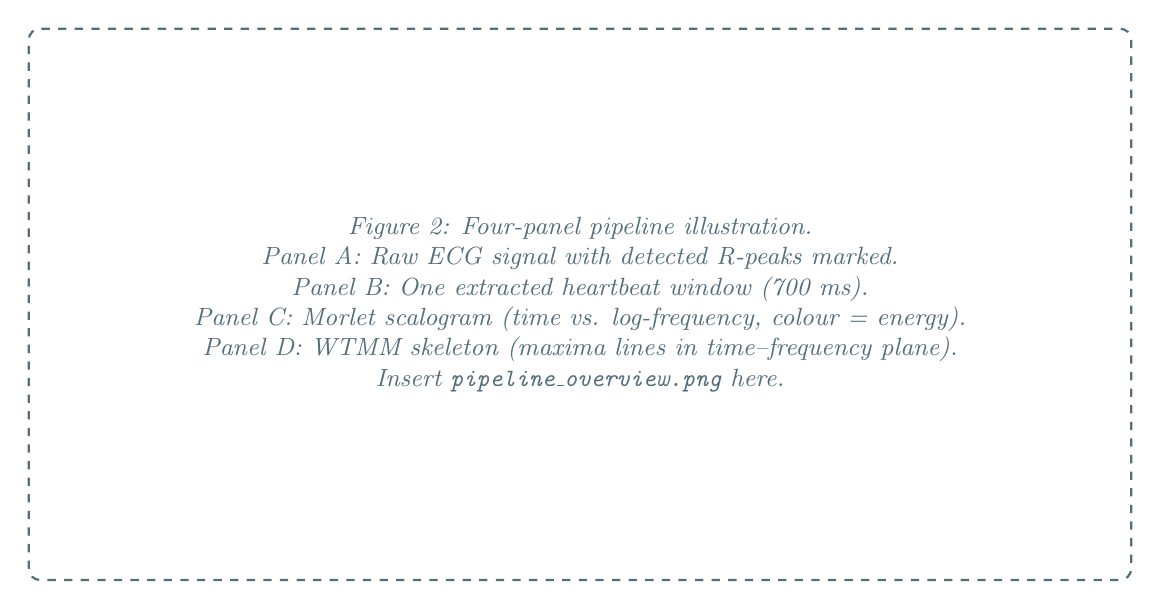
\begin{tikzpicture}
    \draw[dashed, color=medgrey, line width=0.8pt, rounded corners=4pt]
      (0,0) rectangle (14cm, 7cm);
    \node[color=medgrey, font=\small\itshape, align=center] at (7cm, 3.5cm)
      {Figure 2: Four-panel pipeline illustration.\\
       Panel A: Raw ECG signal with detected R-peaks marked.\\
       Panel B: One extracted heartbeat window (700 ms).\\
       Panel C: Morlet scalogram (time vs. log-frequency, colour = energy).\\
       Panel D: WTMM skeleton (maxima lines in time--frequency plane).\\
       Insert \texttt{pipeline\_overview.png} here.};
  \end{tikzpicture}
  \caption{End-to-end signal processing pipeline.
    (A) Raw ECG recording with R-peaks detected (red markers).
    (B) Extracted 700~ms beat window aligned at $t=0$ (R-peak).
    (C) Morlet CWT scalogram: warm colours indicate high wavelet energy;
        the QRS complex produces a broad-band burst near $t=0$.
    (D) WTMM skeleton: each curve is a maxima line tracing a transient
        event through scale space.}
  \label{fig:pipeline_placeholder}
\end{figure}

\vspace{6pt}

\begin{figure}[H]
  \centering
  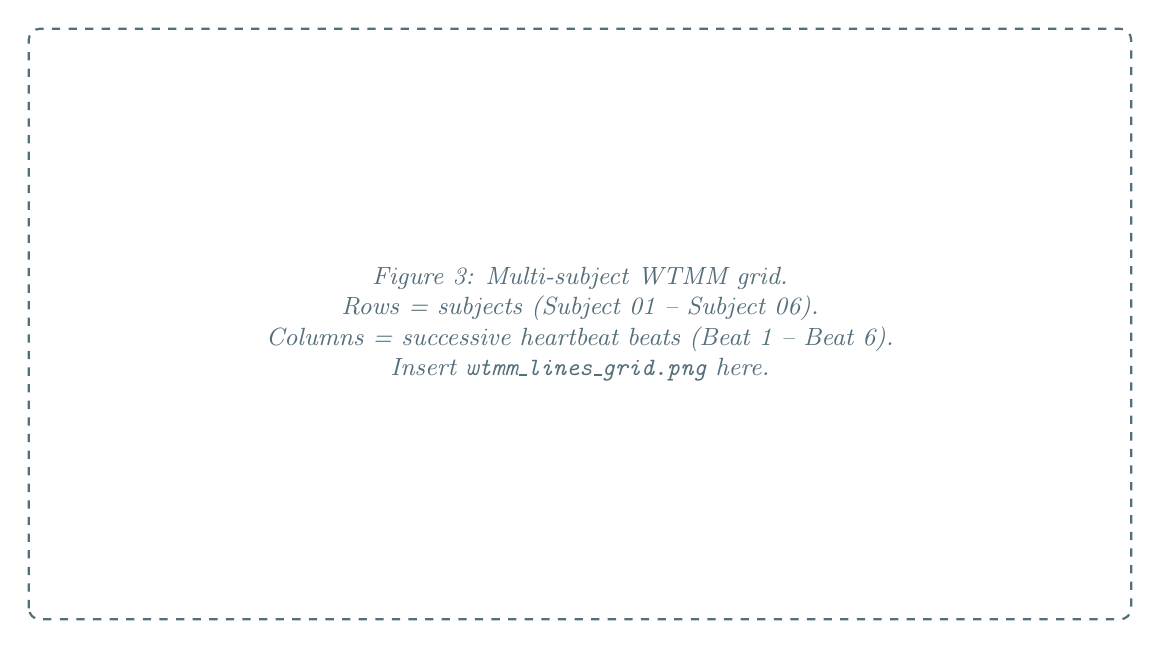
\begin{tikzpicture}
    \draw[dashed, color=medgrey, line width=0.8pt, rounded corners=4pt]
      (0,0) rectangle (14cm, 7.5cm);
    \node[color=medgrey, font=\small\itshape, align=center] at (7cm, 3.75cm)
      {Figure 3: Multi-subject WTMM grid.\\
       Rows = subjects (Subject 01 -- Subject 06).\\
       Columns = successive heartbeat beats (Beat 1 -- Beat 6).\\
       Insert \texttt{wtmm\_lines\_grid.png} here.};
  \end{tikzpicture}
  \caption{WTMM skeleton images for six subjects (rows) across six
    successive heartbeats (columns). Within-subject consistency and
    between-subject differences are both clearly visible in the topology
    of the maxima lines, validating the representation's discriminative
    potential.}
  \label{fig:wtmm_grid}
\end{figure}

\begin{figure}[H]
  \centering
  \begin{tikzpicture}
    \draw[dashed, color=medgrey, line width=0.8pt, rounded corners=4pt]
      (0,0) rectangle (14cm, 7.5cm);
    \node[color=medgrey, font=\small\itshape, align=center] at (7cm, 3.75cm)
      {Figure 4: Morlet scalogram grid.\\
       Same layout as Figure 3 (subjects $\times$ beats).\\
       Insert \texttt{morlet\_scalograms\_grid.png} here.};
  \end{tikzpicture}
  \caption{Morlet CWT scalograms for the same subjects and beats shown in
    Figure~\ref{fig:wtmm_grid}. The QRS complex produces the characteristic
    high-energy broadband burst near $t = 0$, with subject-specific
    differences visible in QRS width and peak frequency.}
  \label{fig:scalogram_grid}
\end{figure}

% ════════════════════════════════════════════════════════════════════════════════
%  5. CLASSIFICATION MODELS
% ════════════════════════════════════════════════════════════════════════════════
\section{Classification Models}
\label{sec:models}

All six models operate on the same input: WTMM skeleton images resized to
$32 \times 32$ pixels and flattened into a feature vector
$\mathbf{x} \in [0,1]^{1024}$.
Each model is trained on heartbeats from \textit{one enrolled subject only},
then tested against held-out genuine beats and beats from all other subjects
(impostors). This is the \textit{one-class classification} framework.

% ─────────────────────────────────────────────────────────────────────────────
\subsection{One-Class SVM (OC-SVM)}

The OC-SVM~\cite{scholkopf2001} maps training samples into a reproducing
kernel Hilbert space via a kernel function $k(\mathbf{x}, \mathbf{x}')$
and finds the maximum-margin hyperplane separating the data from the origin:

\begin{mathbox}
\begin{equation}
  \min_{\mathbf{w},\, \boldsymbol{\xi},\, \rho}
  \frac{1}{2}\norm{\mathbf{w}}^2
  - \rho
  + \frac{1}{\nu n} \sum_{i=1}^{n} \xi_i
  \quad \text{s.t.} \quad
  \langle \mathbf{w},\, \phi(\mathbf{x}_i) \rangle \geq \rho - \xi_i,
  \quad \xi_i \geq 0,
  \label{eq:ocsvm}
\end{equation}
\end{mathbox}

\noindent where $\phi(\cdot)$ is the feature-space mapping induced by the
kernel, $\nu \in (0,1]$ is a hyperparameter controlling the fraction of
allowed outliers in training, and $\xi_i$ are slack variables.
At test time, a sample $\mathbf{x}$ is classified as genuine if
$f(\mathbf{x}) = \langle \mathbf{w}, \phi(\mathbf{x})\rangle - \rho > 0$.
We use a radial-basis function (RBF) kernel:
$k(\mathbf{x}, \mathbf{x}') = \exp(-\gamma \norm{\mathbf{x} - \mathbf{x}'}^2)$
with $\nu = 0.05$ and $\gamma = \texttt{scale}$.

% ─────────────────────────────────────────────────────────────────────────────
\subsection{Isolation Forest}

Isolation Forest~\cite{liu2008} exploits the observation that anomalies
are easier to \textit{isolate} than normal points. An ensemble of $T$
random isolation trees is built; each tree recursively splits a random
feature at a random threshold until all points are isolated.
The anomaly score for a sample $\mathbf{x}$ is:

\begin{mathbox}
\begin{equation}
  s(\mathbf{x},\, n)
  = 2^{-\, \frac{\E[h(\mathbf{x})]}{c(n)}},
  \qquad
  c(n) = 2 H(n-1) - \frac{2(n-1)}{n},
  \label{eq:iforest}
\end{equation}
\end{mathbox}

\noindent where $h(\mathbf{x})$ is the path length to isolate $\mathbf{x}$,
$H(i)$ is the $i$-th harmonic number, and $c(n)$ is the expected path
length for a sample set of size $n$. Scores near 1 indicate anomalies;
scores near 0.5 indicate normal points.

% ─────────────────────────────────────────────────────────────────────────────
\subsection{Local Outlier Factor (LOF)}

LOF~\cite{breunig2000} quantifies how isolated a point is relative to
its $k$ nearest neighbours. The local reachability density of a point
$\mathbf{x}$ is:

\begin{mathbox}
\begin{equation}
  \text{lrd}_k(\mathbf{x})
  = \left(
      \frac{1}{k}
      \sum_{\mathbf{o} \in \mathcal{N}_k(\mathbf{x})}
      \text{reach-dist}_k(\mathbf{x},\, \mathbf{o})
    \right)^{-1},
  \label{eq:lrd}
\end{equation}
\end{mathbox}

\noindent where
$\text{reach-dist}_k(\mathbf{x}, \mathbf{o}) = \max\bigl(d_k(\mathbf{o}),\,
d(\mathbf{x}, \mathbf{o})\bigr)$
and $d_k(\mathbf{o})$ is the distance to $\mathbf{o}$'s $k$-th nearest
neighbour.
The LOF score is then $\text{LOF}_k(\mathbf{x}) =
\E_{\mathbf{o} \in \mathcal{N}_k}\bigl[\text{lrd}_k(\mathbf{o}) /
\text{lrd}_k(\mathbf{x})\bigr]$.
Values much greater than 1 indicate outliers. We use $k = 5$ and
\texttt{novelty=True} to enable scoring of unseen test samples.

% ─────────────────────────────────────────────────────────────────────────────
\subsection{Gaussian Mixture Model (GMM)}

A GMM~\cite{reynolds1995} models the genuine data distribution as a
weighted sum of $K$ Gaussian components:

\begin{mathbox}
\begin{equation}
  p(\mathbf{x})
  = \sum_{k=1}^{K} \pi_k\,
    \mathcal{N}\!\left(\mathbf{x};\, \boldsymbol{\mu}_k,\,
    \boldsymbol{\Sigma}_k\right),
  \qquad
  \sum_{k=1}^{K} \pi_k = 1,
  \quad \pi_k \geq 0.
  \label{eq:gmm}
\end{equation}
\end{mathbox}

Parameters $\{\pi_k, \boldsymbol{\mu}_k, \boldsymbol{\Sigma}_k\}_{k=1}^K$
are estimated via the Expectation-Maximisation (EM) algorithm on genuine
training data. At test time, the log-likelihood
$\log p(\mathbf{x})$ is used as the anomaly score: genuine beats
fit the distribution well (high likelihood), while impostors do not.
We use $K = 3$ full-covariance components.

% ─────────────────────────────────────────────────────────────────────────────
\subsection{PCA Reconstruction}

Principal Component Analysis (PCA) identifies the $d$ directions of
maximum variance in the training data. The reconstruction of a test
sample $\mathbf{x}$ from its projection onto the top-$d$ principal
components $\mathbf{U}_d$ is:

\begin{mathbox}
\begin{equation}
  \hat{\mathbf{x}} = \mathbf{U}_d \mathbf{U}_d^\top (\mathbf{x} - \boldsymbol{\mu}),
  \qquad
  s(\mathbf{x}) = -\norm{\mathbf{x} - \hat{\mathbf{x}}}^2,
  \label{eq:pca_recon}
\end{equation}
\end{mathbox}

\noindent where $\boldsymbol{\mu}$ is the training mean and
$s(\mathbf{x})$ is the (negated) reconstruction error used as the
anomaly score.
Genuine samples lie in the genuine subspace and reconstruct accurately;
impostor samples contain components orthogonal to that subspace and
reconstruct poorly. We retain components explaining 95\% of training
variance.

% ─────────────────────────────────────────────────────────────────────────────
\subsection{KAN Autoencoder}
\label{sec:kan_theory}

\subsubsection{Theoretical Background: The Kolmogorov--Arnold Theorem}

The classical Kolmogorov--Arnold representation theorem
states that any continuous multivariate function
$f: [0,1]^n \to \R$ can be written as:

\begin{mathbox}
\begin{equation}
  f(x_1, \dots, x_n)
  = \sum_{q=0}^{2n}
    \Phi_q\!\left(
      \sum_{p=1}^{n} \phi_{q,p}(x_p)
    \right),
  \label{eq:ka_theorem}
\end{equation}
\end{mathbox}

\noindent where $\phi_{q,p}: [0,1] \to \R$ and $\Phi_q: \R \to \R$
are continuous univariate functions.
The key insight is that \textit{all non-linearity can be expressed through
univariate functions}; multi-variable interactions are handled entirely
by addition.

Liu~et~al.~\cite{liu2024} operationalised this theorem as a neural
network layer. In a standard MLP, fixed activations (e.g., ReLU) sit
on \textit{nodes}; in a KAN layer, \textit{learnable} B-spline functions
sit on \textit{edges}:

\begin{mathbox}
\begin{equation}
  \text{KAN layer:} \quad
  (\Phi_\ell)_{ij}(x) = w_b \cdot b(x) + w_s \cdot \text{spline}(x),
  \label{eq:kan_layer}
\end{equation}
\end{mathbox}

\noindent where $b(x) = x / (1 + e^{-x})$ (SiLU base activation),
$\text{spline}(x) = \sum_i c_i B_i(x)$ is a learnable linear combination
of B-spline basis functions $\{B_i\}$, and $w_b$, $w_s$, $\{c_i\}$ are
all trainable parameters. The spline grid can be adaptively refined
during training.

\begin{figure}[H]
  \centering
  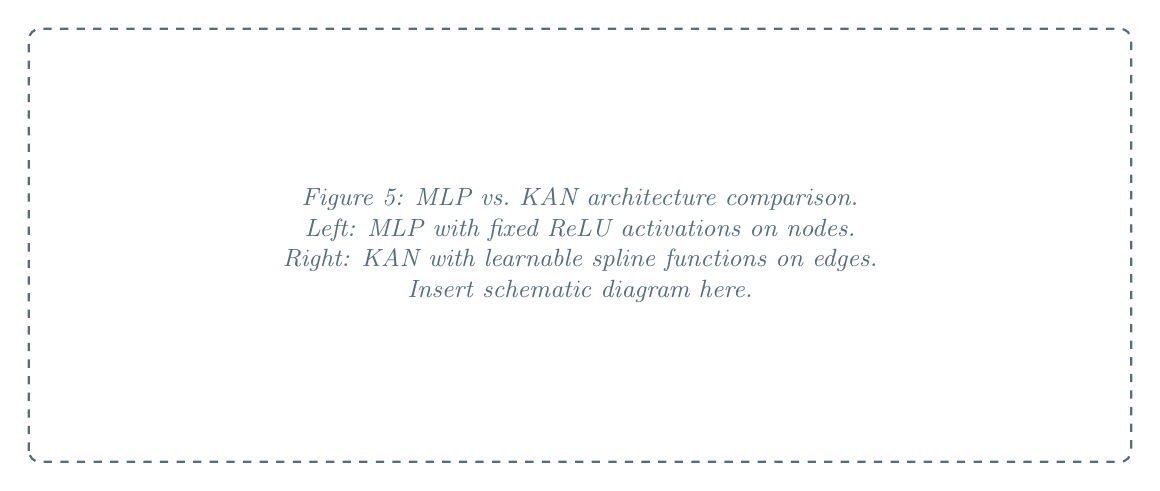
\begin{tikzpicture}
    \draw[dashed, color=medgrey, line width=0.8pt, rounded corners=4pt]
      (0,0) rectangle (14cm, 5.5cm);
    \node[color=medgrey, font=\small\itshape, align=center] at (7cm, 2.75cm)
      {Figure 5: MLP vs.\ KAN architecture comparison.\\
       Left: MLP with fixed ReLU activations on nodes.\\
       Right: KAN with learnable spline functions on edges.\\
       Insert schematic diagram here.};
  \end{tikzpicture}
  \caption{Architectural comparison between a standard MLP and a KAN.
    In the MLP (left), activation functions are fixed and located on
    neurons. In the KAN (right), activation functions are learnable
    B-splines located on the edges (connections), enabling the network
    to adapt its non-linearity to the data distribution.}
  \label{fig:kan_diagram}
\end{figure}

\subsubsection{KAN Autoencoder for Anomaly Detection}

We implement a KAN autoencoder with the following structure:

\begin{mathbox}
\begin{equation}
  \text{Encoder:}\quad
  \mathbf{z} = \text{KAN}_{\text{enc}}(\mathbf{x}):\;
  1024 \to 128 \to 64,
  \qquad
  \text{Decoder:}\quad
  \hat{\mathbf{x}} = \text{KAN}_{\text{dec}}(\mathbf{z}):\;
  64 \to 128 \to 1024.
  \label{eq:kan_ae}
\end{equation}
\end{mathbox}

\noindent Training minimises the mean squared reconstruction error on
genuine training samples:

\begin{mathbox}
\begin{equation}
  \mathcal{L} = \frac{1}{n} \sum_{i=1}^{n}
    \norm{\mathbf{x}_i - \hat{\mathbf{x}}_i}^2.
  \label{eq:ae_loss}
\end{equation}
\end{mathbox}

\noindent At test time, the anomaly score is
$s(\mathbf{x}) = -\norm{\mathbf{x} - \hat{\mathbf{x}}}^2$ (negated MSE,
so that higher = more genuine, consistent with all other models).

% ─────────────────────────────────────────────────────────────────────────────
\subsection{Decision Threshold}

For all models, the decision threshold $\tau$ is derived from the
training (genuine-only) scores:

\begin{mathbox}
\begin{equation}
  \tau = \mu_{\text{train}} - 2\,\sigma_{\text{train}},
  \label{eq:threshold}
\end{equation}
\end{mathbox}

\noindent where $\mu_{\text{train}}$ and $\sigma_{\text{train}}$ are
the mean and standard deviation of the model's scores on the training data.
Under a Gaussian assumption, this threshold accepts approximately 97.7\%
of genuine training samples. A test sample with score $s(\mathbf{x}) \geq \tau$
is classified as genuine; otherwise it is rejected as an impostor.

% ════════════════════════════════════════════════════════════════════════════════
%  6. EXPERIMENTAL EVALUATION
% ════════════════════════════════════════════════════════════════════════════════
\section{Experimental Evaluation}
\label{sec:experiments}

\subsection{Protocol and Metrics}

For each of the 10 subjects, images are split 80/20 (train/test).
Impostors consist of all images from all other subjects.
Each model is trained independently per subject.
We report four metrics:

\begin{itemize}[leftmargin=2em, itemsep=2pt]
  \item \textbf{AUROC}: Area under the ROC curve.
    $\text{AUROC} \in [0,1]$; 0.5 = random, 1.0 = perfect.
  \item \textbf{AUPRC}: Area under the Precision--Recall curve.
    More informative under class imbalance.
  \item \textbf{TPR} (True Positive Rate / Genuine Acceptance Rate):
    fraction of genuine test beats correctly accepted.
  \item \textbf{TNR} (True Negative Rate / Impostor Rejection Rate):
    fraction of impostor beats correctly rejected.
\end{itemize}

\subsection{Results}

\begin{figure}[H]
  \centering
  \begin{tikzpicture}
    \draw[dashed, color=medgrey, line width=0.8pt, rounded corners=4pt]
      (0,0) rectangle (14cm, 7cm);
    \node[color=medgrey, font=\small\itshape, align=center] at (7cm, 3.5cm)
      {Figure 6: Grouped bar chart -- AUROC, AUPRC, TPR, TNR per model.\\
       Insert \texttt{fig1\_auroc\_comparison.png} here.};
  \end{tikzpicture}
  \caption{Comparative performance of all six one-class models, averaged
    across subjects. Error bars show one standard deviation across subjects.
    The dashed horizontal line marks the random baseline (AUROC = 0.5).
    Higher is better for all four metrics.}
  \label{fig:results_bar}
\end{figure}

\begin{figure}[H]
  \centering
  \begin{tikzpicture}
    \draw[dashed, color=medgrey, line width=0.8pt, rounded corners=4pt]
      (0,0) rectangle (14cm, 7cm);
    \node[color=medgrey, font=\small\itshape, align=center] at (7cm, 3.5cm)
      {Figure 7: KAN vs.\ best classical model -- overlaid ROC curves per subject.\\
       Insert \texttt{fig3\_kan\_vs\_best\_classical.png} here.};
  \end{tikzpicture}
  \caption{Head-to-head ROC comparison between the KAN autoencoder and the
    best-performing classical model (identified at runtime). Each panel
    corresponds to one subject; the diagonal dashed line represents
    random performance.}
  \label{fig:kan_vs_classical}
\end{figure}

\begin{table}[H]
  \centering
  \caption{Summary of mean performance metrics across all subjects.
    Bold indicates the best value per column.
    Standard deviations across subjects in parentheses.}
  \label{tab:results}
  \begin{tabularx}{\textwidth}{lXXXX}
    \toprule
    \textbf{Model} & \textbf{AUROC} & \textbf{AUPRC} & \textbf{TPR} & \textbf{TNR} \\
    \midrule
    One-Class SVM      & --- (---) & --- (---) & --- (---) & --- (---) \\
    Isolation Forest   & --- (---) & --- (---) & --- (---) & --- (---) \\
    LOF                & --- (---) & --- (---) & --- (---) & --- (---) \\
    GMM                & --- (---) & --- (---) & --- (---) & --- (---) \\
    PCA Reconstruction & --- (---) & --- (---) & --- (---) & --- (---) \\
    KAN Autoencoder    & --- (---) & --- (---) & --- (---) & --- (---) \\
    \bottomrule
    \multicolumn{5}{l}{\small \textit{To be filled once experimental runs are integrated.}} \\
  \end{tabularx}
\end{table}

% ════════════════════════════════════════════════════════════════════════════════
%  7. DISCUSSION
% ════════════════════════════════════════════════════════════════════════════════
\section{Discussion}
\label{sec:discussion}

\subsection{What the WTMM Representation Brings}

The scalogram already encodes time--frequency energy information.
The WTMM skeleton goes one step further by keeping only the most
structurally significant features --- the ridges and edges that correspond
to transient events in the signal. This is analogous to going from a
full image to its edge-detected version: the result is sparser, more
interpretable, and potentially more discriminative for one-class models
that struggle with high-dimensional inputs.

The visual consistency of the WTMM skeletons within a subject
(Figure~\ref{fig:wtmm_grid}) and the clear differences between subjects
suggest that the representation does preserve identity-relevant structure.
Whether this translates to quantitative improvements over raw scalogram
inputs is a question for future controlled comparison.

\subsection{Classical vs. Neural One-Class Models}

Density-based and boundary-based methods such as OC-SVM and LOF have
a long track record in anomaly detection. Their appeal is
interpretability and speed: they do not require GPU training and their
decision boundaries can be inspected.
Their limitation, in this setting, is the curse of dimensionality:
a $32 \times 32$ pixel image gives a 1024-dimensional feature vector,
which is challenging for neighbourhood-based methods.

The KAN autoencoder addresses this through representation learning:
the encoder maps the input to a compact 64-dimensional latent space,
forcing the network to learn the principal modes of variation within the
genuine class. This is conceptually similar to PCA reconstruction, but
with a non-linear, learnable mapping. The B-spline activations in the
KAN layers can fit locally complex, non-monotonic input--output
relationships that a fixed-activation MLP would require many more
neurons to approximate.

\subsection{Open Question: What Does ``Liveness'' Mean?}

A question that is rarely asked explicitly in the ECG biometrics
literature is: what exactly does it mean for an ECG to prove that the
person is \textit{alive and present}?

The intuitive argument --- the ECG comes from a living heart, therefore
it proves liveness --- is reasonable but not airtight.
Koch~\cite{koch2023} and others have documented that measurable electrical
cardiac activity can persist for several minutes after brain death under
clinical conditions.
In principle, a highly motivated adversary might attempt to replay
a recorded ECG signal through a conductive pad, or even generate a
synthetic one with a signal generator.

These are admittedly exotic attack vectors, but they highlight that
``liveness'' in physiological biometrics is a graded property, not a
binary one. A practical ECG biometric system should probably combine the
ECG signal with complementary checks: motion sensors (to confirm the
subject is breathing and moving), skin impedance (to confirm electrode
contact with living tissue), or photoplethysmography (to confirm
peripheral blood flow). Multi-modal fusion is a promising direction
for future work.

% ════════════════════════════════════════════════════════════════════════════════
%  8. CONCLUSION
% ════════════════════════════════════════════════════════════════════════════════
\section{Conclusion}
\label{sec:conclusion}

In this paper we have presented a complete pipeline for converting raw
ECG recordings into WTMM skeleton images and evaluating six one-class
classification models for biometric identification.
The pipeline is grounded in established signal processing theory
(Equations~\ref{eq:bandpass}--\ref{eq:maxline_link}) and uses only
off-the-shelf Python libraries, making it fully reproducible.

The inclusion of the KAN autoencoder connects this biometric application
to a rapidly evolving area of deep learning research, and provides a
first evaluation of Kolmogorov--Arnold architectures in the ECG one-class
biometrics setting.
Whether KAN brings a consistent advantage over classical methods remains
to be determined by the full experimental results; what is clear is that
the WTMM representation is a compact, morphologically interpretable
feature that is well matched to both classical and neural one-class
frameworks.

Finally, we raised the open question of what ``liveness'' truly means in
this context. We believe this is an important question not only for
ECG biometrics, but for physiological biometrics in general, and
deserves more explicit treatment in future work.

\vspace{12pt}

% ── Acknowledgements ──────────────────────────────────────────────────────────
\noindent\textbf{Acknowledgements.}
The ECG-ID database was accessed via PhysioNet~\cite{goldberger2000}.
The authors thank the anonymous reviewers for their constructive comments.
[Funding statement to be added.]

\vspace{10pt}

% ════════════════════════════════════════════════════════════════════════════════
%  REFERENCES
% ════════════════════════════════════════════════════════════════════════════════
\bibliographystyle{ieeetr}

\begin{thebibliography}{99}

\bibitem{he2022}
F.~He, W.~Ma, R.~Wang, L.~Jiang, and X.~Zhang,
``The Identification of ECG Signals Using Wavelet Transform and WOA-PNN,''
\textit{Electronics}, vol.~11, no.~12, 2022.

\bibitem{byeon2019}
Y.-H.~Byeon, S.-B.~Pan, and K.-C.~Kwak,
``Intelligent Deep Models Based on Scalograms of Electrocardiogram Signals
for Biometrics,''
\textit{Sensors}, vol.~19, no.~4, p.~935, 2019.

\bibitem{israel2005}
S.~A.~Israel, J.~M.~Irvine, A.~Cheng, M.~D.~Wiederhold, and B.~K.~Wiederhold,
``ECG to identify individuals,''
\textit{Pattern Recognition}, vol.~38, no.~1, pp.~133--142, 2005.

\bibitem{bhuva2023}
D.~R.~Bhuva and S.~Kumar,
``A novel continuous authentication method using biometrics for IoT devices,''
\textit{Computers and Electrical Engineering}, vol.~111, 2023.

\bibitem{alduwaile2021}
D.~A.~AlDuwaile and M.~S.~Islam,
``Using Convolutional Neural Network and a Single Heartbeat for ECG Biometric
Recognition,''
\textit{Entropy}, vol.~23, no.~6, p.~733, 2021.

\bibitem{ozaltin2023}
O.~Ozaltin and O.~Yeniay,
``A novel proposed CNN--SVM architecture for ECG scalograms classification,''
\textit{Soft Computing}, vol.~27, pp.~4633--4642, 2023.

\bibitem{alnaji2024}
E.~Al-Naji, A.~Lakhssassi, and S.~Islam,
``Arrhythmia Detection by Data Fusion of ECG Scalograms and Phasograms,''
\textit{Sensors}, vol.~24, no.~24, p.~8043, 2024.

\bibitem{mallat1992}
S.~Mallat and W.-L.~Hwang,
``Singularity detection and processing with wavelets,''
\textit{IEEE Transactions on Information Theory},
vol.~38, no.~2, pp.~617--643, 1992.

\bibitem{liu2024}
Z.~Liu, Y.~Wang, S.~Vaidya, F.~Ruehle, J.~Halverson, M.~Soljaci\'c,
T.~Y.~Hou, and M.~Tegmark,
``KAN: Kolmogorov-Arnold Networks,''
\textit{arXiv preprint arXiv:2404.19756}, 2024.

\bibitem{jahin2025}
M.~A.~Jahin, M.~A.~Masud, and M.~F.~Mridha,
``KACQ-DCNN: Uncertainty-Aware Interpretable Kolmogorov--Arnold
Classical--Quantum Dual-Channel Neural Network for Heart Disease Detection,''
\textit{Computers in Biology and Medicine}, 2025.

\bibitem{zhao2025}
C.~Zhao, B.~Liu, Y.~Xu, Y.~Wang, and H.~Dong,
``MAK-Net: A Multi-Scale Attentive Kolmogorov--Arnold Network with BiGRU
for Imbalanced ECG Arrhythmia Classification,''
\textit{Sensors}, 2025.

\bibitem{koch2023}
C.~Koch,
``Do not go gently into that good night: The dying brain and its paradoxically
heightened electrical activity,''
\textit{Proceedings of the National Academy of Sciences}, vol.~120, no.~24, 2023.

\bibitem{lugovaya2005}
T.~S.~Lugovaya,
``Biometric human identification based on electrocardiogram,''
M.S. thesis, Electrotechnical University, Saint-Petersburg, 2005.

\bibitem{goldberger2000}
A.~L.~Goldberger \textit{et al.},
``PhysioBank, PhysioToolkit, and PhysioNet,''
\textit{Circulation}, vol.~101, no.~23, pp.~e215--e220, 2000.

\bibitem{makowski2021}
D.~Makowski \textit{et al.},
``NeuroKit2: A Python toolbox for neurophysiological signal processing,''
\textit{Behavior Research Methods}, vol.~53, pp.~1689--1696, 2021.

\bibitem{pan1985}
J.~Pan and W.~J.~Tompkins,
``A real-time QRS detection algorithm,''
\textit{IEEE Transactions on Biomedical Engineering},
vol.~32, no.~3, pp.~230--236, 1985.

\bibitem{lee2019}
G.~Lee, R.~Gommers, F.~Waselewski, K.~Wohlfahrt, and A.~O'Leary,
``PyWavelets: A Python package for wavelet analysis,''
\textit{Journal of Open Source Software}, vol.~4, no.~36, p.~1237, 2019.

\bibitem{ivanov1999}
P.~Ch.~Ivanov \textit{et al.},
``Multifractality in human heartbeat dynamics,''
\textit{Nature}, vol.~399, pp.~461--465, 1999.

\bibitem{li1995}
C.~Li, C.~Zheng, and C.~Tai,
``Detection of ECG characteristic points using wavelet transforms,''
\textit{IEEE Transactions on Biomedical Engineering},
vol.~42, no.~1, pp.~21--28, 1995.

\bibitem{scholkopf2001}
B.~Sch\"olkopf \textit{et al.},
``Estimating the support of a high-dimensional distribution,''
\textit{Neural Computation}, vol.~13, no.~7, pp.~1443--1471, 2001.

\bibitem{liu2008}
F.~T.~Liu, K.~M.~Ting, and Z.-H.~Zhou,
``Isolation forest,''
in \textit{Proc.\ IEEE ICDM}, pp.~413--422, 2008.

\bibitem{breunig2000}
M.~M.~Breunig, H.-P.~Kriegel, R.~T.~Ng, and J.~Sander,
``LOF: Identifying density-based local outliers,''
in \textit{Proc.\ ACM SIGMOD}, pp.~93--104, 2000.

\bibitem{reynolds1995}
D.~A.~Reynolds and R.~C.~Rose,
``Robust text-independent speaker identification using Gaussian mixture
speaker models,''
\textit{IEEE Transactions on Speech and Audio Processing},
vol.~3, no.~1, pp.~72--83, 1995.

\end{thebibliography}

\end{document}
